%! Author = Sujal Singh
%! Date = 12/3/23

% Preamble
\documentclass[11pt]{beamer}
\title[Derivation for mass-energy equivalence] {Derivation for mass-energy equivalence $[E = mc^2]$}
\author[Chitransh, Divyanshi, Prashant...]
{\(|\) Chitransh Koshta \(|\) Divyanshi Panchal \(|\) Prashant Pulkit \(|\)\\\(|\) Priyanshu Raj
    \(|\) Sujal Singh \(|\)}
\date[Priyanshu, Sujal]{}

\usetheme{Madrid}
\usecolortheme{beaver}
\setbeamertemplate{navigation symbols}{}
\setbeamertemplate{frametitle continuation}[from second][]

% Packages
\usepackage{amsmath}
\usepackage{cancel}
\usepackage{tikz}

\usetikzlibrary{arrows.meta,arrows}

% Document
\begin{document}
    \begin{frame}{Physics Presentation (Group 9)}
        \begin{center}
            %! suppress = FileNotFound
            
\includegraphics[width=80pt]{logo}
        \end{center}\vspace*{-20pt}
        \maketitle
    \end{frame}

    \begin{frame}[t]{Introduction}
        \begin{minipage}[t]{0.65\textwidth}
            In 1905, Albert Einstein published a paper titled \textit{``On the Electrodynamics of Moving Bodies''},
            in which he described the \textbf{Special Theory of Relativity}.\ Using this theory, he derived an equation
            showing mass-energy equivalence:
            \begin{align*}
                E = mc^2
            \end{align*}
            This implied that mass and energy are one and the same and are interchangeable.\\[10pt]
            Let us derive this equation.
        \end{minipage}
        \begin{minipage}[t]{0.05\textwidth}
            ~
        \end{minipage}
        \begin{minipage}[t]{0.1\textwidth}
            \begin{center}
                \vspace*{-10pt}
                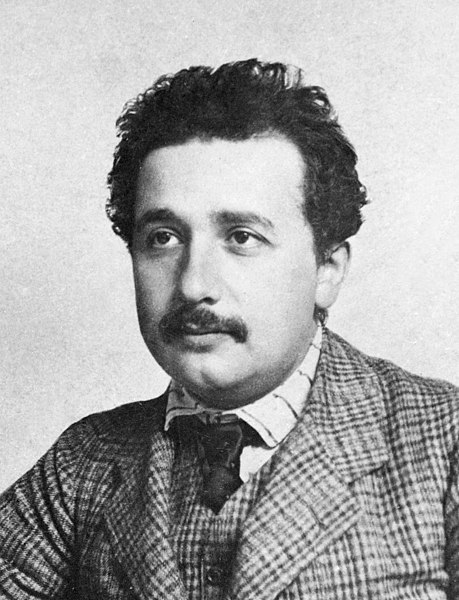
\includegraphics[width=100pt]{albert}
            \end{center}
        \end{minipage}
    \end{frame}
\end{document}